\documentclass[letter,12pt]{article}
\usepackage[utf8]{inputenc}
\usepackage{tabu}
\usepackage{tabularx}
\usepackage{multirow}
\usepackage[none]{hyphenat} 
\usepackage{fancyhdr}
\usepackage{graphicx}
\usepackage{tabu}
\usepackage{tabularx}
\usepackage{multirow}
\usepackage[none]{hyphenat} %No corte palabras
\usepackage{cite} 			% para contraer referencias

% idioma
\usepackage[utf8]{inputenc}
\usepackage[spanish]{babel}

% subitems enumerated
\usepackage[pointedenum]{paralist} 

%tablas
\usepackage{booktabs}

%rotar tablas
\usepackage{rotating}

%color tablas
\usepackage{colortbl}
\usepackage{comment}
\usepackage{enumitem}
\usepackage{hyperref}
\usepackage{cite}
\hypersetup{
    colorlinks=true,
    linkcolor=blue,
    filecolor=magenta,      
    urlcolor=blue,
}

%espaciado
\usepackage{setspace}
\onehalfspacing
\setlength{\parindent}{0pt}
\setlength{\parskip}{2.0ex plus0.5ex minus0.2ex}


%margenes según n. icontec
\usepackage{vmargin}
\setmarginsrb           
    { 2.5cm}  % left margin
    { 2.5cm}  % top margcm
    { 2.5cm}  % right margcm
    { 2.5cm}  % bottom margcm
    {   5pt}  % head height
    { 2cm  }  % head sep
    {   9pt}  % foot height
    { 1.0cm}  % foot sep

%Secciones: 
% 1. Datos Personales Estudiantes [Hecho]
% 2. Modalidad [Hecho]
% 3. Titulo [Hecho]
% 4. Introducción [Hecho]
% 5. Planteamiento del Problema TODO
% 6. Objetivo General [Hecho]
% 7. Objetivos Específicos [Hecho]
% 8. Metodología [Hecho]
% 9. Cronograma TODO
% 10. Presupuestos y Fuentes de Financiación [Hecho]
% 11. Bibliografía TODO
\spacing{1.2}
\pagestyle{fancy}
\fancyhf{}
\rhead{
\includegraphics[width=1.6cm]{isc.jpg}}
\chead{ \textbf{
\hspace{1.5cm}UNIVERSIDAD TECNOLÓGICA DE PEREIRA
\\\hspace{1.5cm}FACULTAD DE INGENIERÍAS
\\\hspace{1.5cm}Programa de Ingeniería de Sistemas y Computación}
}
\lhead{
\includegraphics[width=3.3cm]{identificador-horizontal.jpg}}
\rfoot{\thepage}
\renewcommand{\headrulewidth}{0pt}


\begin{document}
\sloppy %No corte palabras
\renewcommand{\arraystretch}{1.1} %Alto de las celdas
%------------------------------------------
%Datos Personales
\begin{center}
\begin{tabular}{|p{5.5cm}|p{9.5cm}|}
\hline
\multicolumn{2}{|c|}{\textbf{1. Datos Personales del Estudiante}}\\
\hline
\textbf{Código} & 1115421345 \\
\hline
\textbf{Nombres} & Héctor Fabio\\
\hline
\textbf{Apellidos} & Jiménez Saldarriaga\\
\hline
\textbf{email} & hfjimenez@utp.edu.co \\
\hline
\textbf{Teléfonos} & +573127400482 +573175548245 \\
\hline
\end{tabular}
\end{center}

%Director de Proyecto de Grado
\begin{center}
\begin{tabular}{|p{5.5cm}|p{9.5cm}|}
\hline
\textbf{Nombre del Director} & Ramiro Andrés Barrios Valencia \\
\hline
\textbf{VoBo Director} &  \\
\hline
\textbf{VoBo Comité Curricular} &  \\
\hline
\end{tabular}
\end{center}
%------------------------------------------
%Modalidad
\begin{center}
\begin{tabular}{|p{5.5cm}|p{8.5cm}|p{0.5cm}|}
\hline
\multicolumn{3}{|c|}{\textbf{2. Modalidad}}\\
\hline
\multirow{3}{5cm}{\textbf{1. Trabajo de Investigación Formativa}} & Proyecto de Investigación &  \\ \cline{2-3}
& Proyecto de Aplicación &  \textbf{X}\\ \cline{2-3}
& Monografía &  \\ 
\hline
\multirow{3}{5cm}{\textbf{2. Práctica de Extensión}} & Práctica Universitaria &  \\ \cline{2-3}
& Emprendimiento Empresarial &  \\ \cline{2-3}
& Proyecto Social &  \\
\hline
\end{tabular}
\end{center}
\newpage
%------------------------------------------
%Titulo del Trabajo de Grado
\begin{center}
\begin{tabular}{|p{15.5cm}|}
\hline
\multicolumn{1}{|c|}{ \textbf{3. Título del Trabajo de Grado}}\\
\hline
Despliegues Automaticos de Infraestructuras HPC multinucleo y multimaquina con maquinas virtuales utilizando Vagrant\\
\hline
\end{tabular}
\end{center}
    
%---------------------------------------
%Introducción
\begin{center}
\begin{tabular}{|p{15.5cm}|}
\hline
\multicolumn{1}{|c|}{ \textbf{4. Introducción} }\\
\hline
Introduccion de Infraestructure as a Code, Utilización de maquinas virtuales para entornos educativos, construccion de cluster .\\
\hline
\end{tabular}
\end{center}
%------------------------------------------
%Problema
\begin{center}
\begin{tabular}{|p{15.5cm}|}
\hline
\multicolumn{1}{|c|}{ \textbf{5. Planteamiento del Problema} }\\
\hline
\textbf{Descripción}
Que problemas resuelve la infraestructura como codigo, ataques que resuelve vagrant\\
\hline
\end{tabular}
\end{center}

%------------------------------------------
%Objetivo General
\begin{center}
\begin{tabular}{|p{15.5cm}|}
\hline
\multicolumn{1}{|c|}{ \textbf{6. Objetivo General}}\\
\hline
Cual es el objetivo general, generar guias para el laboratorio de HPC. 
Que cosas podria aprender un estudiante con vagrant ?
Cambiar Objetivos\\
\hline
\end{tabular}
\end{center}

%------------------------------------------
%Objetivos Específicos

\begin{center}
\begin{tabular}{|p{15.5cm}|}
\hline
\multicolumn{1}{|c|}{ \textbf{7. Objetivos Específicos}}\\
\hline
\begin{itemize}
	\item Implementar alguna de las técnicas para el análisis de logs y eventos que cumplan el estándar RFC3164.
	\item Desarrollar e implementar un sistema de archivos distribuido en el cluster.
	\item Implementar un cluster utilizando contenedores para garantizar el aislamiento y protección de los datos recolectados.
    \item Realizar pruebas de desempeño frente a otras posibles soluciones del mismo costo.
\end{itemize} \\
\hline
\end{tabular}
\end{center}

%------------------------------------------
%Metodología

\begin{center}
\begin{tabular}{|p{15.5cm}|}
\hline
\multicolumn{1}{|c|}{ \textbf{8. Metodología} }\\
\hline
\textbf{Fases de la Metodología}
    \begin{enumerate}
        \item Investigación y Análisis:
        xx
        \item Formulación
		xx
        \end{enumerate}\\
        
\hline
\end{tabular}
\end{center}

\begin{center}
\begin{tabular}{|p{15.5cm}|}
\hline    
        
        3. Pruebas
  
    \textbf{Hipótesis}
    Será posible obtener una reducción costos de hardware para la recolección, pre-procesamiento, filtrado y análisis de acontecimientos obtenidos de múltiples fuentes que generen eventos o logs que cumplan con el estándar RFC3164. 
    \par
    
    \textbf{Variables}
    \begin{itemize}
        \item Costos de Hardware
        \item Performance del cluster
    \end{itemize} \\

    
    \textbf{Diseño Metodológico}
    \begin{itemize}
        \item  Mediante Diagrama de Gantt, Se recogen las tareas y actividades que componen al
proyecto y se asocian a un cronograma para de esta forma dejar reflejado la
duración de las actividades y del proyecto y de cada uno de las entregas. No será
muy útil gracias a su simplicidad y que el proyecto no será muy cambiante por lo
que la estructura de cronograma de actividades no debería verse afectado durante
el desarrollo de las actividades que conforman al proyecto.

  El enfoque y método seguido para la ejecución de este proyecto es \textit{“aprender haciéndoló”}, parte desde la construcción y ensamblaje de los componentes de las
SBCs hasta la parametrización y configuración de cada una de las tecnologías y software implicados, todo ello llevado a cabo desde un punto de vista práctico.
        
        
    \end{itemize}\\  
        
\hline
\end{tabular}
\end{center}

\begin{center}
\begin{tabular}{|p{15.5cm}|}
\hline
    
    \begin{itemize}
        
        \item Tipo de investigación
        
        Basados en los puntos anteriores se considera que éste es un Proyecto de investigación; ya que se pretende que por medio de la obtención de nuevos conocimientos por medio de investigación, se obtenga un resultado o entregable después de la culminación. 
    
        En esta investigación se utilizará un enfoque cuantitativo. Además de que se empleará el método científico.
        
        \item Estrategias
        
        Se llevará a cabo un conjunto de pruebas sobre el sistema, para establecer si cumple con las estimaciones del proyecto y si es un funcional.
    \end{itemize}\\  

\hline
\end{tabular}
\end{center}

%------------------------------------------
%Cronograma

\begin{center}
\begin{tabular}{|p{15.5cm}|}
\hline
\multicolumn{1}{|c|}{ \textbf{9. Cronograma}}\\
\hline

A continuación se describe un esquema de las actividades que se desarrollarán durante el proyecto, cada una con su respectiva duración:
    
    \begin{center}
    \begin{tabular}{|p{9.5cm}|p{0.4cm}|p{0.4cm}|p{0.4cm}|p{0.4cm}|p{0.4cm}|p{0.4cm}|}
    \hline
    \multicolumn{7}{|c|}{\textbf{Cronograma de Actividades}}\\
    \hline
    \textbf{Actividad / Tiempo(Meses)} & \textbf{1} & \textbf{2} & \textit{\textbf{3}} & \textbf{4} & \textbf{5} & \textbf{6} \\
    \hline
    Documentación e investigación detallada de eletronica en tarjetas SBC & X &   &   &   &   &   \\
    \hline
    Estado del arte de Sistemas operativos para tarjetas SBC & X &   &   &   &   &   \\
    \hline
    Elaboración de propuesta de trabajo & X &   &   &   &   &   \\
    \hline
    Investigación sobre las metodologías a aplicar en el proyecto &   & X &   &   &   &   \\
    \hline
    Análisis de arquitecturas de software, sistemas de archivos,  contenedores distribuidos&   & X &   &   &   &   \\
    \hline
    Elección de las técnicas que serán aplicadas &   &   & X &   &   &   \\
    \hline
    Investigar sobre cada técnica &   &   & X &   &   &   \\
    \hline
    Desarrollo de algoritmo &   &   &   & X &   &   \\
    \hline
    Pruebas sobre algoritmo &   &   &   & X &   &   \\
    \hline
    Elaboración de informe final &   &   &   &   & X &   \\
    \hline
    Entrega &   &   &   &   &   & X \\
    \hline
    \end{tabular}
    \end{center} \\

\hline
\end{tabular}
\end{center}


\begin{center}
\begin{tabular}{|p{15.5cm}|}
\hline
\multicolumn{1}{|c|}{ \textbf{10. Presupuesto y Fuentes de Financiación}}\\
\hline

\textbf{Recursos Humanos}
\begin{itemize}
    \item Director de proyecto.
    \item Laboratorio Sirius CIDT
    \item Cluster Lovelace
    \item Grupo de Investigación Sirius. \par
    Ingeniería de Sistemas y Computación. Universidad Tecnológica de Pereira.
\end{itemize}\\
\hline
\end{tabular}
\end{center}
\begin{center}
\begin{tabular}{|p{15.5cm}|}
\hline
	A continuación un valor estimado para los recursos considerados en el proyecto:
	\begin{center}
    \begin{tabular}{|p{2.5cm}|p{3cm}|p{2cm}|p{2cm}|p{3cm}|}
    \hline
    \textbf{Recurso Humano} & \textbf{Costo(Peso Colombiano) / Hora } & \textbf{Número Horas} & \textbf{Total} & \textbf{Fuente Financiadora} \\
    \hline
    Investigador (Tesista1) & 5.700 & 200 & 1.140.000 & Universidad \\
    \hline    \hline
    Director / Asesor & 30.000 & 80 & 2.400.000 & Universidad \\
    \hline
    \textbf{Compra o Alquiler de Maquinaria y Equipos} & \textbf{Costo(Peso Colombiano) } & \textbf{Cantidad} & \textbf{Total} & \textbf{Fuente Financiadora} \\
    \hline
    Computador Dell, procesador i5, 1TB DD y 10GB RAM & 1.900.000 & 1 & 1.900.000 & Tesista 1 \\
    \hline

    \textbf{Fungibles} & \textbf{Costo(Peso Colombiano) } & \textbf{Cantidad} & \textbf{Total} & \textbf{Fuente Financiadora} \\
    \hline
    Papelería y otros & 50.000 &  & 50.000 & Tesista \\
    \hline
    Servicios públicos & 95.000 &  & 95.000 & Tesista1 \\
    \hline
    \textbf{Costo Total del Proyecto} &  &  & 7.650.000 &  \\
    \hline
    \end{tabular}
    \end{center}\\
\hline
\end{tabular}
\end{center}
%------------------------------------------
%Bibliografía
\begin{center}
\begin{tabular}{|p{15.5cm}|}
\hline
\multicolumn{1}{|c|}{ \textbf{11. Bibliografía}}\\
\hline
\\
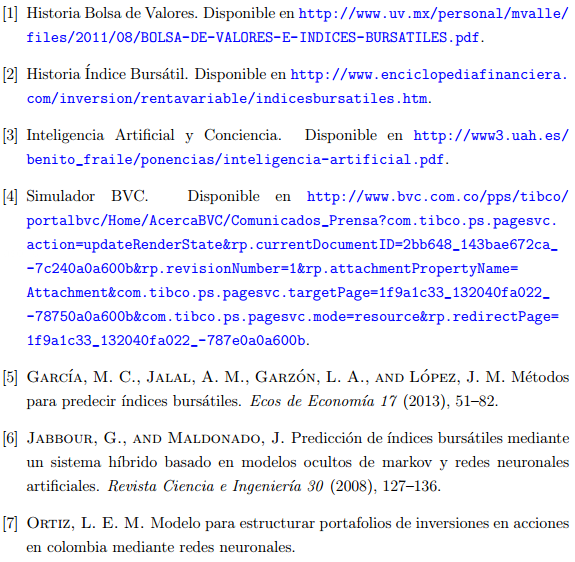
\includegraphics[width=0.95\textwidth]{ref.png}
\\
\hline
\end{tabular}
\end{center}
%------------------------------------------
\end{document}